\documentclass[11pt,a4paper]{article}

% ===== Packages =====
\usepackage{graphicx}   % 圖片
\usepackage{amsmath}    % 數學公式
\usepackage{booktabs}   % 表格線條
\usepackage{geometry}   % 頁邊距
\usepackage{float}
\usepackage{graphicx}   % 插圖功能
\usepackage{caption}
\usepackage{subcaption} % 讓多圖排列用
\usepackage[a4paper,margin=1in]{geometry}
\geometry{margin=1in}

% ===== Document =====
\begin{document}

% ===== Title Page =====
\title{Lab 2: Pipelined RISC-V Processor}
\author{Student ID: 314551138}
\date{10 13, 2025}
\maketitle

% ===== Sections =====
\section{Introduction}
This lab extends the original five-stage pipelined RISC-V processor into a seven-stage design
by adding two extra stages (X2 and X3) to support a pipelined \texttt{mul}/\texttt{div} unit.
The main objectives are to complete the control logic, implement full bypassing to minimize stalls,
and ensure correct hazard detection between arithmetic and memory operations.
Through custom tests and random-delay simulations, we verified that the modified hazard control
effectively balances correctness and performance under complex dependency chains.
Finally, benchmark results were collected to compare cycle counts and IPC
across the \texttt{riscvstall}, \texttt{riscvbyp}, and \texttt{riscvlong} processors,
demonstrating the performance improvement achieved by bypassing and pipeline extension.

\section{Design}

\subsection{riscvstall}
Objective 1 focused on enhancing the control unit in riscvstall-CoreCtrl.v.
All necessary datapath connections were already defined, so the task mainly involved
completing the control signal table for each instruction and verifying their interaction
with the five-stage pipeline (F–D–X–M–W).
We implemented all remaining rv32i and rv32m entries, including arithmetic, memory,
branch, and jump instructions. The design pipelines all control signals from Decode to their
target stages instead of using a traditional FSM, ensuring one-cycle latency consistency.
A conservative stalling policy was used to guarantee correctness by fully preventing data hazards
before bypassing was introduced in later objectives.
\subsection{riscvbyp}

In this stage, the processor was extended to support full bypassing across the X, M, and W stages,
allowing dependent instructions to proceed without unnecessary stalls.
The datapath was modified to include two 2-bit bypass selectors (\texttt{rs1\_byp\_sel\_Dhl} and \texttt{rs2\_byp\_sel\_Dhl})
that determine whether each source operand in Decode comes from the register file, the X-stage ALU result,
the M-stage execution result, or the W-stage writeback value.
The control logic in \texttt{riscvbyp-CoreCtrl.v} generates these selectors based on data dependency detection signals
(\texttt{rs*\_X/M/W\_byp\_Dhl}) computed from register indices and write enables.

To ensure correctness under memory latency, a refined stall condition was introduced:
the pipeline now stalls only for true load-use hazards detected between D–X and D–M stages,
identified using an \texttt{is\_load} flag pipelined through X and M.
This replaced the original conservative stall policy, which previously stalled on all data dependencies.
Additional safeguards were added to prevent timeout issues observed under random-delay simulations,
especially when \texttt{lw/sw} instructions overlapped with other memory requests.

The datapath in \texttt{riscvbyp-CoreDpath.v} was updated accordingly with new bypass multiplexers
feeding both ALU operands and memory store data.  
Simulation confirmed correct forwarding behavior across dependent instruction pairs,
and benchmark results showed significant cycle count reduction compared to the stall-only version.

\subsection{riscvlong }
In the objective4, we extended the original 5-stage RISC-V pipeline (P→F→D→X→M→W) into a 7-stage version (P→F→D→X→M→X2→X3→W) to integrate a fully pipelined 4-stage Mul/Div unit. The first two stages of the Mul/Div pipeline overlap with the X and M stages, while two additional stages (X2 and X3) were inserted before Writeback to accommodate the extended latency. 

To maintain correctness across the pipeline, we modified the control logic to propagate Mul/Div-related control signals through all additional stages. Signals such as \texttt{is\_md}, \texttt{is\_load}, \texttt{muldiv\_mux\_sel}, and \texttt{execute\_mux\_sel} were all extended to X2 and X3 stages to ensure the proper timing alignment between datapath operations and control signals.

In the datapath, we implemented multi-level bypassing to reduce unnecessary stalls. Specifically, both source operands (\texttt{rs1} and \texttt{rs2}) can now bypass from five possible sources: X, M, X2, X3, and W. This allows instructions dependent on ALU results to proceed without stalling, except in cases of load-use or inter-Mul/Div-use hazards.

During the debugging phase, we encountered a critical issue where several instructions became corrupted in the pipeline and produced undefined values (“x” contamination) during simulation. Using \textbf{GTKWave}, we traced the signal propagation stage by stage and discovered that the control signal \texttt{execute\_mux\_sel} itself turned into an undefined (‘x’) value as soon as the pipeline entered the Execute stage. This caused the downstream signals — including ALU output and pipeline registers — to propagate the invalid state, leading to incorrect behavior and contamination of XXXXXXXX(undefined) in whole pipeline.

After several attempts to isolate the cause, we consulted \textbf{AI} for further reasoning support. Through analysis, we learned that the original control logic:

\begin{verbatim}
wire execute_mux_sel_Dhl = cs[`RISCV_INST_MSG_EX_SEL];
\end{verbatim}

was inherited from the 5-stage pipeline version, where the \texttt{EX\_SEL} field correctly determined whether the ALU or the iterative Mul/Div unit should provide the output in the \textbf{X stage}. However, in the new 7-stage pipeline that integrates a 4-stage pipelined Mul/Div unit, the result is only valid in the \textbf{X3 stage}. As a result, the original \texttt{EX\_SEL} no longer aligned with the actual timing of the datapath — \texttt{execute\_mux\_sel} became indeterminate before any valid data existed, directly causing the “x contamination.”

To fix this, we modified the control logic as follows:

\begin{verbatim}
wire execute_mux_sel_Dhl = cs[`RISCV_INST_MSG_MULDIV_EN];
\end{verbatim}

By binding the selection signal directly to \texttt{MULDIV\_EN}, we ensured that all Mul/Div instructions carry this tag consistently from the \textbf{Decode stage} through \textbf{X → M → X2 → X3}, where the actual result becomes valid. This adjustment effectively synchronizes the control and datapath timing, prevents premature selection, and stabilizes all intermediate signals.

After the change, we re-ran the simulation and used GTKWave to verify the result. All signals were stable, \texttt{execute\_mux\_sel} maintained a consistent value throughout the pipeline, and all random-delay test cases passed successfully.

\section{Testing Methodology}
\subsection{Custom tests(riscv-custom)}
This custom test is designed to verify the correctness of pipeline behavior
when \texttt{lw} and \texttt{sw} memory operations are interleaved with arithmetic instructions
such as \texttt{mul}, \texttt{div}, and \texttt{add}.
During the random delay testing phase, a significant amount of time was spent
debugging time-out issues related to \texttt{lw}/\texttt{sw} instructions.
Further investigation revealed that the cause was an overly strict
hazard control condition on load-use and memory-related dependencies,
which unnecessarily stalled the pipeline and delayed instruction retirement.

To address this, the \texttt{custom\_tests.S} program focuses on
interleaving multiple \texttt{lw}, \texttt{sw}, and arithmetic operations,
aiming to ensure that:
\begin{itemize}
  \item load-use hazards are detected correctly and stalls are inserted only when necessary;
  \item store-followed-by-load sequences read back the most recent data correctly;
  \item the pipeline maintains correct results and timing when multiple functional units are active concurrently.
\end{itemize}


Overall, this test validates that the revised hazard control logic
properly relaxes unnecessary stall conditions while maintaining correct execution order
under mixed memory and arithmetic workloads.
In addition, the \texttt{mul} extension instructions were also tested
with boundary and corner-case operands to confirm
the correctness of high/low product handling and signed/unsigned multiplication behavior.


\section{Evaluation and Discussion}

Below table summarizes the performance results for all four benchmarks across the three processor implementations. Each design was functionally verified to pass all tests, and cycle counts and IPC values were collected using the provided simulation framework.

\begin{table}[h!]
\centering
\caption{Performance comparison of riscvstall, riscvbyp, and riscvlong processors.}
\label{tab:lab2-eval}
\begin{tabular}{l|l|r|r|r}
\hline
\textbf{Processor} & \textbf{Benchmark} & \textbf{Cycles} & \textbf{Instructions} & \textbf{IPC} \\ \hline
riscvstall & vvadd & 1778 & 1064 & 0.598 \\
riscvbyp   & vvadd & 1535 & 1064 & 0.693 \\
riscvlong  & vvadd & 1537 & 1066 & 0.694 \\ \hline
riscvstall & masked-filter & 21032 & 6964 & 0.331 \\
riscvbyp   & masked-filter & 18051 & 6964 & 0.386 \\
riscvlong  & masked-filter & 10397 & 6966 & 0.670 \\ \hline
riscvstall & cmplx-mult & 18687 & 2949 & 0.158 \\
riscvbyp   & cmplx-mult & 16876 & 2949 & 0.175 \\
riscvlong  & cmplx-mult & 4203  & 2951 & 0.702 \\ \hline
riscvstall & bin-search & 3258  & 1126 & 0.346 \\
riscvbyp   & bin-search & 1633  & 1126 & 0.690 \\
riscvlong  & bin-search & 1635  & 1128 & 0.690 \\ \hline
\end{tabular}
\end{table}

\noindent
\textbf{Analysis.} The experimental results clearly demonstrate that pipelining and bypassing significantly improve performance. The baseline \texttt{riscvstall} processor, which resolves all hazards via stalling, achieves the lowest IPC across all benchmarks. Introducing bypassing in \texttt{riscvbyp} eliminates unnecessary stalls between dependent ALU instructions, improving IPC by 15--20\%. The \texttt{riscvlong} processor, integrating a pipelined multiply/divide unit, achieves the highest throughput, with IPC gains up to 4$\times$ in the compute-intensive \texttt{cmplx-mult} benchmark.

Bypassing is most effective in arithmetic-heavy workloads (\texttt{vvadd}, \texttt{bin-search}), while load-use hazards still limit \texttt{masked-filter}. The pipelined MulDiv unit in \texttt{riscvlong} further improves parallelism by overlapping long-latency operations with independent instructions, demonstrating reduced total cycles and enhanced IPC in complex multiplication and masked filter.

Overall, these results confirm the expected performance hierarchy:
\[
\texttt{riscvstall} < \texttt{riscvbyp} < \texttt{riscvlong}.
\]


\section{Figures}


\begin{figure}[htbp]
    \centering

    % 第一張圖：riscvbyp
    \begin{subfigure}{0.95\linewidth}
        \centering
        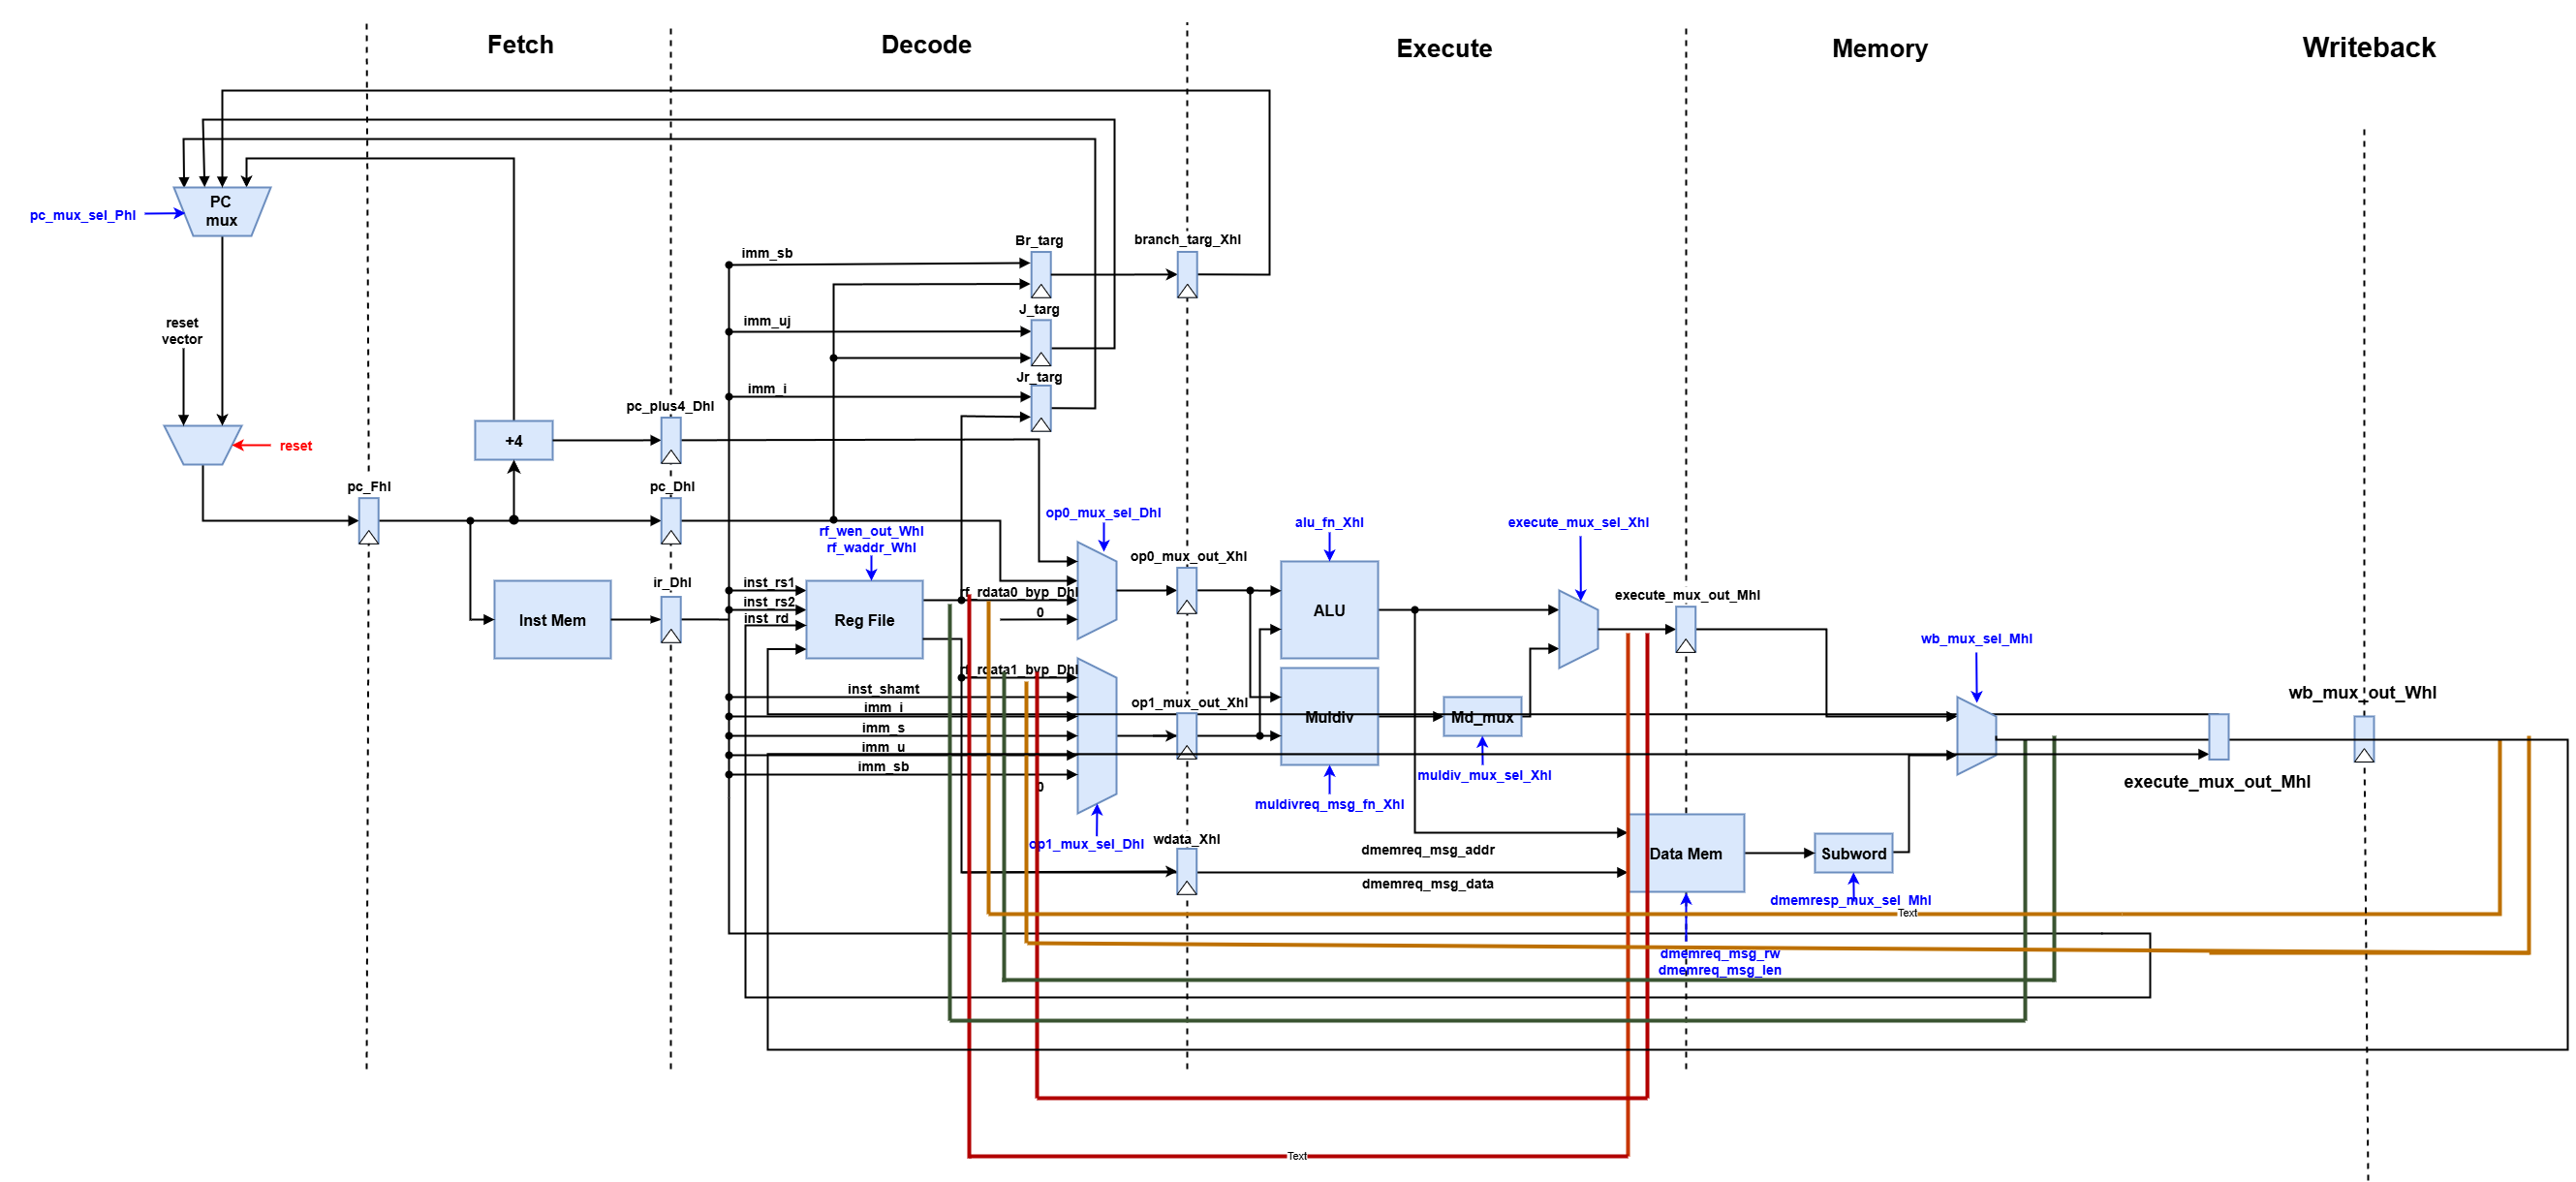
\includegraphics[width=\linewidth]{riscvbyp.png}
        \caption{5-Stage RISC-V Datapath (riscvbyp)}
        \label{fig:riscvbyp}
    \end{subfigure}

    \vspace{1em}

    % 第二張圖：riscvlong
    \begin{subfigure}{0.95\linewidth}
        \centering
        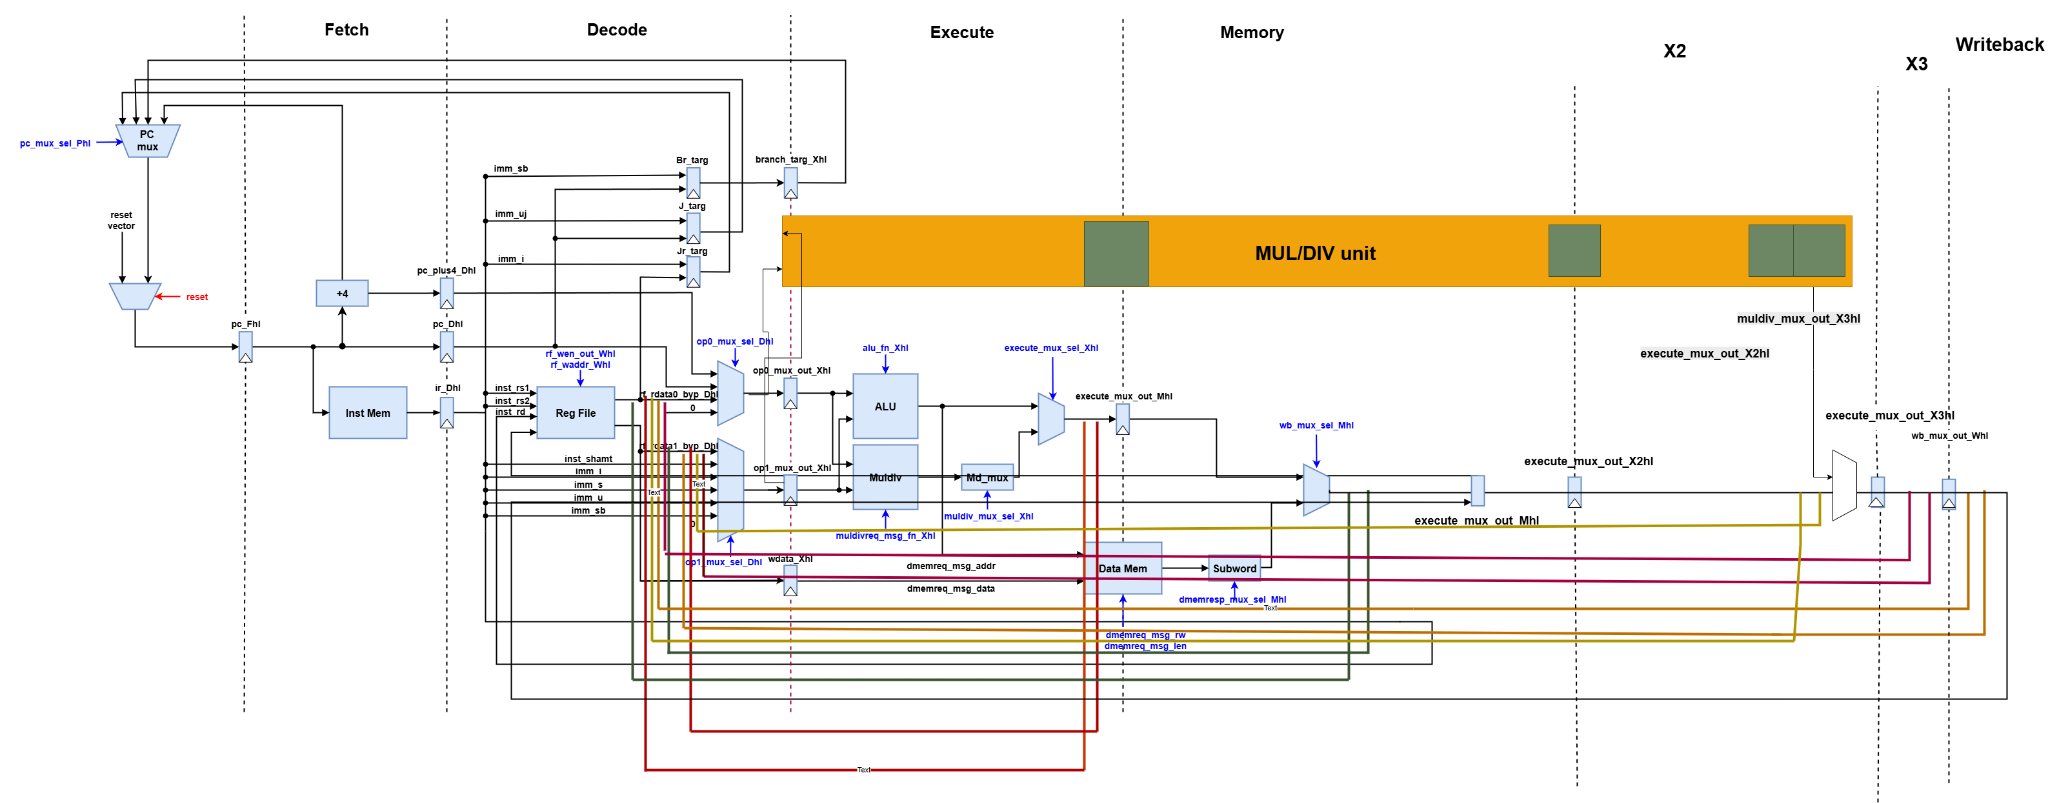
\includegraphics[width=\linewidth]{riscvlong.png}
        \caption{7-Stage RISC-V Datapath with Pipelined MUL/DIV (riscvlong)}
        \label{fig:riscvlong}
    \end{subfigure}

    \caption{Comparison of riscvbyp and riscvlong Datapaths}
    \label{fig:riscv_comparison}
\end{figure}



\end{document}
